\documentclass[]{IEEEtran}
% some very useful LaTeX packages include:
%\usepackage{cite}      
\usepackage{graphicx}   
\usepackage{subfigure} 
\usepackage{url}       
\usepackage{amsmath}    
\usepackage{caption2}
% Your document starts here!
\begin{document}

% Define document title and author
	\title{Weekly Report}
	\author{Adviser: Prof. Yang Wen \\Student: Cheng Wensheng\\ Period: 2018.7.8-7.15
	}
	\markboth{Visual Information Processing Group}{}
	\maketitle

% Write abstract here
\begin{abstract}
	This week I mainly put my effort on preparing SAR data and corresponding optical image for the contest.
\end{abstract}

% Each section begins with a \section{title} command
\section{Optical image}
	% \PARstart{}{} creates a tall first letter for this first paragraph
	\PARstart{A}{fter} geocoding the SAR data, we get the corresponding coordinates. Then we can impose the SAR image on Google Earth, besides, Google Earth has the history images at the same time.
	\begin{itemize}
		\item To label the SAR image, we need to slice the original large SAR image to pieces. And we have to get corresponding optical image and slice it the same way. However, you can't export images directly from Google Earth, so this is a problem.
		\item I found one tool which can download Google Earth history images, but it requires about RMB 3,000 to activate. Finally, I found download services on Taobao, and bought corresponding optical image(8 GB) for RMB 40.
		
		Fig.~\ref{fig:mp} is the SAR image. Fig.~\ref{fig:ss} is the optical image.
	\end{itemize}

% Main Part
\section{Image preprocess}
	% LaTeX takes complete care of your document layout ...
	Since the optical image is relatively large(8 GB), I need to find some tools which can handle with it.
	\begin{itemize}
		\item I used to use PIL image lib to slice large images, yet it even didn't work for the SAR image(450 MB), so I turn to OpenCV and it worked for SAR image.
		\item However, OpenCV could only process image whose size is smaller than 2 GB, and after lots of trials, MATLAB works for the optical image(8 GB).
		\item So I upload sliced SAR images and optical images to Baidu Cloud, and wrote a tutorial to help undergraduates students label these images.
	\end{itemize}
\newpage
\begin{figure}[!hbt]
%		 Center the figure.
		\vspace{0.3cm}
%		\hspace{50cm}
		\begin{center}
			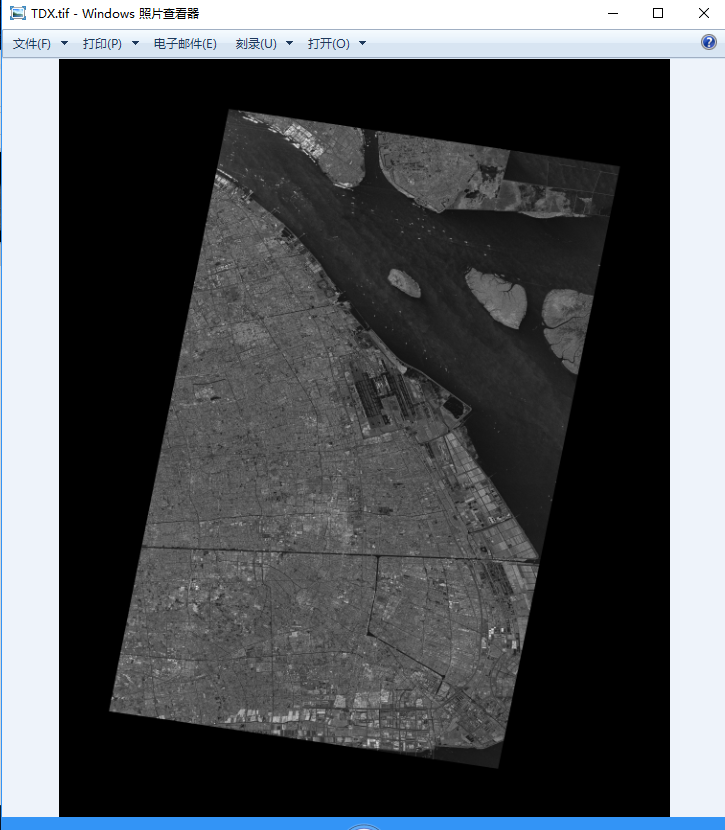
\includegraphics[width=\columnwidth]{sar}
				%		 Create a subtitle for the figure.
			\caption{SAR image(450 MB)}
			\label{fig:mp}
		    \hspace{0.5cm}
			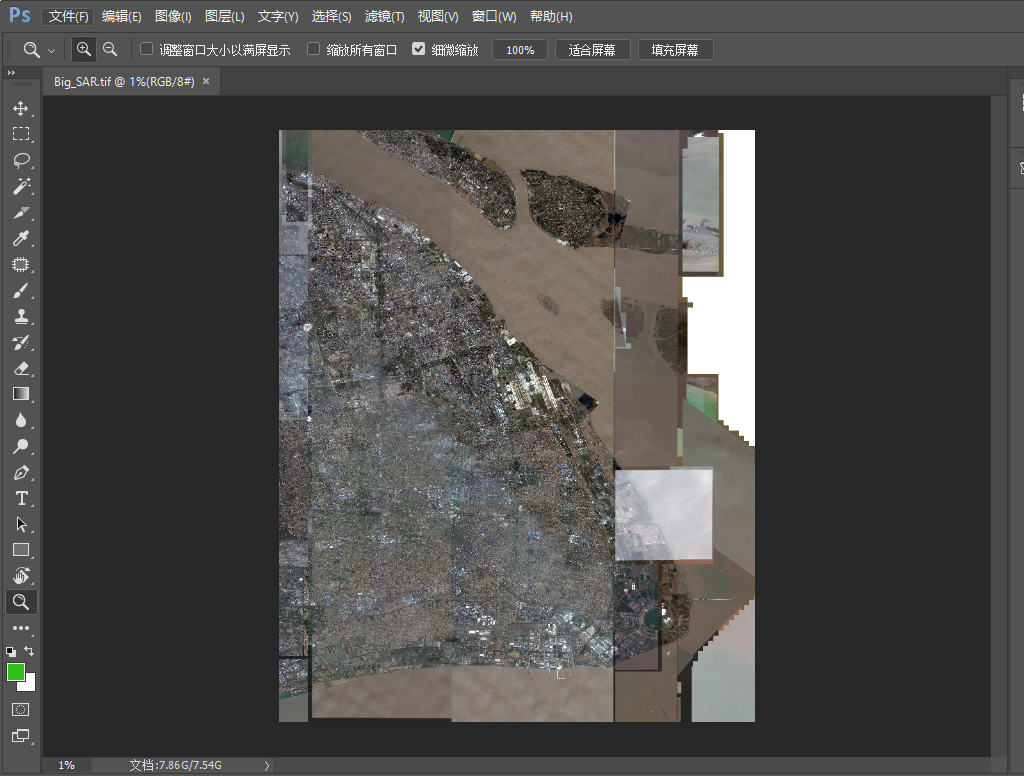
\includegraphics[width=\columnwidth]{opt}
				%Create a subtitle for the figure.
			\caption{Optical image(8 GB)}
			\label{fig:ss}
		\end{center}
	\end{figure}

% Now we need a bibliography:
%\begin{thebibliography}{5}
%
%	%Each item starts with a \bibitem{reference} command and the details thereafter.
%	\bibitem{HOP96} % Transaction paper
%	J.~Hagenauer, E.~Offer, and L.~Papke. Iterative decoding of binary block
%	and convolutional codes. {\em IEEE Trans. Inform. Theory},
%	vol.~42, no.~2, pp.~429–-445, Mar. 1996.
%
%	\bibitem{MJH06} % Conference paper
%	T.~Mayer, H.~Jenkac, and J.~Hagenauer. Turbo base-station cooperation for intercell interference cancellation. {\em IEEE Int. Conf. Commun. (ICC)}, Istanbul, Turkey, pp.~356--361, June 2006.
%
%	\bibitem{Proakis} % Book
%	J.~G.~Proakis. {\em Digital Communications}. McGraw-Hill Book Co.,
%	New York, USA, 3rd edition, 1995.
%
%	\bibitem{talk} % Web document
%	F.~R.~Kschischang. Giving a talk: Guidelines for the Preparation and Presentation of Technical Seminars.
%	\url{http://www.comm.toronto.edu/frank/guide/guide.pdf}.
%
%	\bibitem{5}
%	IEEE Transactions \LaTeX and Microsoft Word Style Files.
%	\url{http://www.ieee.org/web/publications/authors/transjnl/index.html}
%
%\end{thebibliography}

% Your document ends here!
\end{document}